\section{基于openhitls源码的修改}
实验指导书里似乎并没有指明是对openhitls的SM4算法进行优化,所以我们在前面实验中是基于自己实现的SM4算法进行优化的,
在撰写实验报告的时候，我们发现了这个问题，所以在本节我们将对openhitls中的SM4算法进行优化,并测试优化后的性能表现。

我们修改sm4cbc.c文件，加入测速函数，有两种测速方式，一种是对SM4-CBC的CipherUpdate函数进行测试，另一种是对整个加密过程进行测试。
测试核心代码如下:
\begin{lstlisting}[title={openhitls/testcode/demo/sm4cbc.c}]
static int32_t RunBench(CRYPT_EAL_CipherCtx *ctx, const uint8_t *key, uint32_t blockSize)
{
    int32_t ret = CRYPT_SUCCESS;
    uint32_t loops = TOTAL_SIZE / blockSize;

    uint8_t *benchIn = malloc(blockSize);
    uint8_t *benchOut = malloc(blockSize + 16);

    if (benchIn == NULL || benchOut == NULL) {
        printf("malloc failed, blockSize = %u\n", blockSize);
        free(benchIn);
        free(benchOut);
        return -1;
    }

    memset(benchIn, 0x11, blockSize);
    memset(benchOut, 0, blockSize + 16);

    double start = GetTimeSec();

    for (uint32_t loop = 0; loop < loops; loop++) {
        uint8_t benchIv[16] = {0};
        uint32_t benchOutLen = blockSize;
        uint32_t finalLen = 0;

        ret = CRYPT_EAL_CipherInit(ctx, key, 16, benchIv, sizeof(benchIv), true);
        if (ret != CRYPT_SUCCESS) {
            printf("CipherInit failed, error code is %x\n", ret);
            goto EXIT;
        }

        ret = CRYPT_EAL_CipherSetPadding(ctx, CRYPT_PADDING_NONE);
        if (ret != CRYPT_SUCCESS) {
            printf("SetPadding failed, error code is %x\n", ret);
            goto EXIT;
        }

        ret = CRYPT_EAL_CipherUpdate(ctx, benchIn, blockSize, benchOut, &benchOutLen);
        if (ret != CRYPT_SUCCESS) {
            printf("CipherUpdate failed, error code is %x\n", ret);
            goto EXIT;
        }

        ret = CRYPT_EAL_CipherFinal(ctx, benchOut + benchOutLen, &finalLen);
        if (ret != CRYPT_SUCCESS) {
            printf("CipherFinal failed, error code is %x\n", ret);
            goto EXIT;
        }
    }

    double end = GetTimeSec();

    double seconds = end - start;
    double totalMB = (double)TOTAL_SIZE / 1024.0 / 1024.0;
    double speed = totalMB / seconds;

    printf("%8u KB | loops: %6u | time: %.6f s | throughput: %.2f MB/s\n",
           blockSize / 1024, loops, seconds, speed);

EXIT:
    free(benchIn);
    free(benchOut);
    return ret;
}
\end{lstlisting}
结果如下图:
\begin{figure}[H]
    \centering
    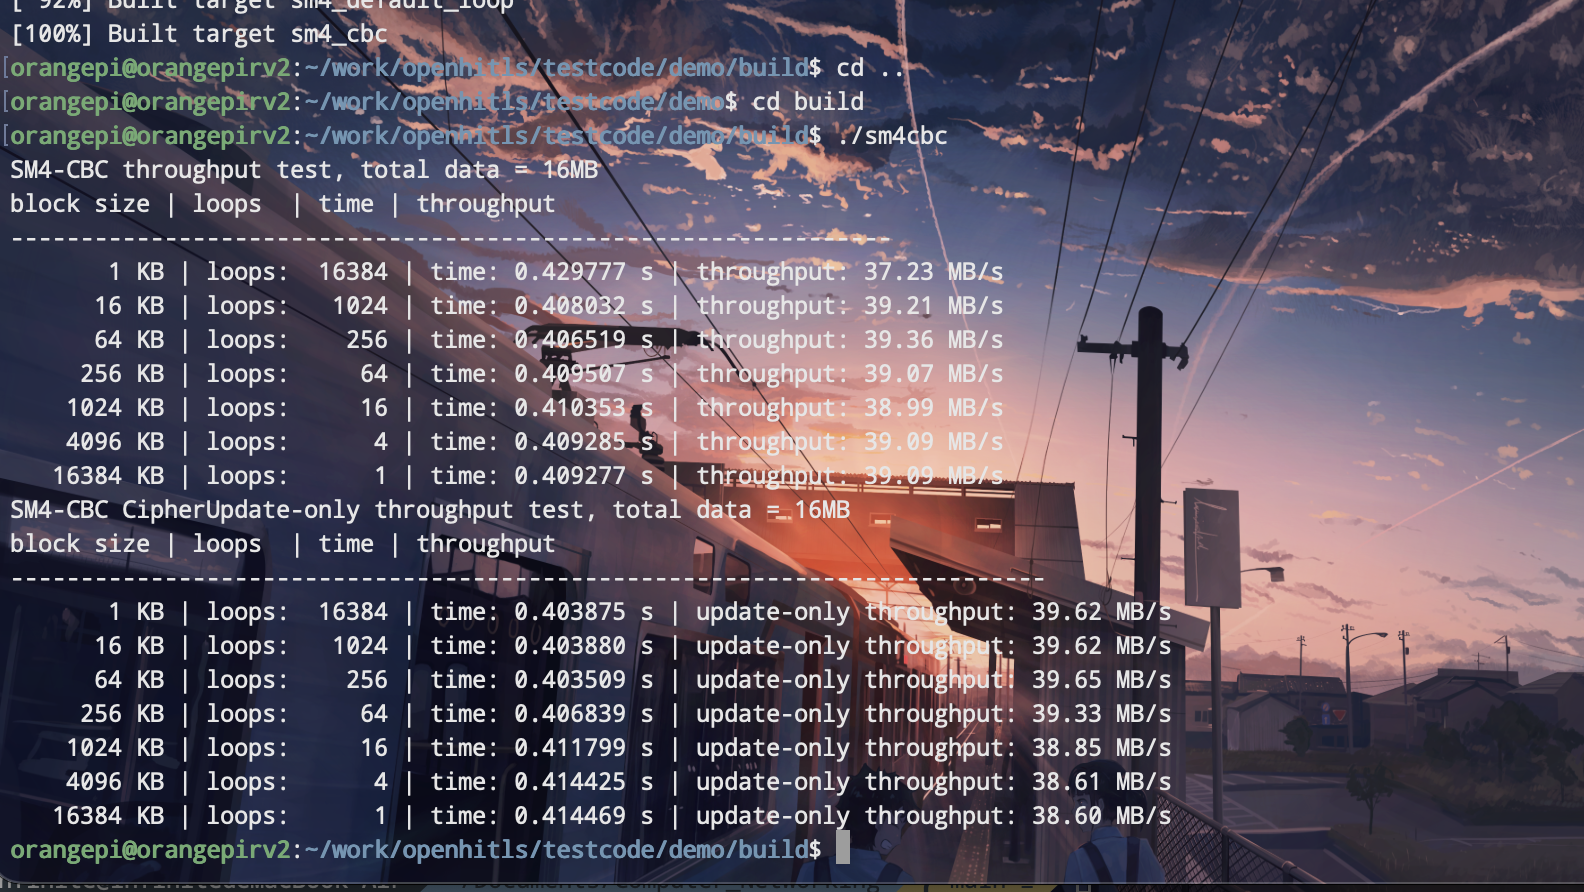
\includegraphics[width = 1\textwidth]{figure/openhitls.png}
    \caption{openhitls SM4-CBC性能测试结果}
\end{figure}

下面我们综合先前的所有优化，在openhitls中叠加实现这些优化，并测试优化后的性能表现。
\subsubsection{循环展开优化}
原代码已经做了4轮循环展开,我们在此基础上进行32轮循环展开
\begin{lstlisting}[title={openhitls/crypto/sm4/src/crypt\_sm4.c}]
#define ENC_ROUND_FUNCTION(t, x0, x1, x2, x3, roundKey, sbox)           \
    for (int i = 0; i < 32; i += 4) {                                   \
        CRYPT_SM4_ROUND((t), (x0), (x1), (x2), (x3), (roundKey)[(i) + 0], sbox);  \
        CRYPT_SM4_ROUND((t), (x1), (x2), (x3), (x0), (roundKey)[(i) + 1], sbox);  \
        CRYPT_SM4_ROUND((t), (x2), (x3), (x0), (x1), (roundKey)[(i) + 2], sbox);  \
        CRYPT_SM4_ROUND((t), (x3), (x0), (x1), (x2), (roundKey)[(i) + 3], sbox);  \
    }
\end{lstlisting}
修改如下
\begin{lstlisting}[title={openhitls/crypto/sm4/src/crypt\_sm4.c}]
#define ENC_ROUND_FUNCTION(t, x0, x1, x2, x3, roundKey, sbox)                 \
    do {                                                                      \
        CRYPT_SM4_ROUND((t), (x0), (x1), (x2), (x3), (roundKey)[0],  sbox);    \
        CRYPT_SM4_ROUND((t), (x1), (x2), (x3), (x0), (roundKey)[1],  sbox);    \
        CRYPT_SM4_ROUND((t), (x2), (x3), (x0), (x1), (roundKey)[2],  sbox);    \
        CRYPT_SM4_ROUND((t), (x3), (x0), (x1), (x2), (roundKey)[3],  sbox);    \
                                                                              \
        CRYPT_SM4_ROUND((t), (x0), (x1), (x2), (x3), (roundKey)[4],  sbox);    \
        CRYPT_SM4_ROUND((t), (x1), (x2), (x3), (x0), (roundKey)[5],  sbox);    \
        CRYPT_SM4_ROUND((t), (x2), (x3), (x0), (x1), (roundKey)[6],  sbox);    \
        CRYPT_SM4_ROUND((t), (x3), (x0), (x1), (x2), (roundKey)[7],  sbox);    \
                                                                              \
        CRYPT_SM4_ROUND((t), (x0), (x1), (x2), (x3), (roundKey)[8],  sbox);    \
        CRYPT_SM4_ROUND((t), (x1), (x2), (x3), (x0), (roundKey)[9],  sbox);    \
        CRYPT_SM4_ROUND((t), (x2), (x3), (x0), (x1), (roundKey)[10], sbox);    \
        CRYPT_SM4_ROUND((t), (x3), (x0), (x1), (x2), (roundKey)[11], sbox);    \
                                                                              \
        CRYPT_SM4_ROUND((t), (x0), (x1), (x2), (x3), (roundKey)[12], sbox);    \
        CRYPT_SM4_ROUND((t), (x1), (x2), (x3), (x0), (roundKey)[13], sbox);    \
        CRYPT_SM4_ROUND((t), (x2), (x3), (x0), (x1), (roundKey)[14], sbox);    \
        CRYPT_SM4_ROUND((t), (x3), (x0), (x1), (x2), (roundKey)[15], sbox);    \
                                                                              \
        CRYPT_SM4_ROUND((t), (x0), (x1), (x2), (x3), (roundKey)[16], sbox);    \
        CRYPT_SM4_ROUND((t), (x1), (x2), (x3), (x0), (roundKey)[17], sbox);    \
        CRYPT_SM4_ROUND((t), (x2), (x3), (x0), (x1), (roundKey)[18], sbox);    \
        CRYPT_SM4_ROUND((t), (x3), (x0), (x1), (x2), (roundKey)[19], sbox);    \
                                                                              \
        CRYPT_SM4_ROUND((t), (x0), (x1), (x2), (x3), (roundKey)[20], sbox);    \
        CRYPT_SM4_ROUND((t), (x1), (x2), (x3), (x0), (roundKey)[21], sbox);    \
        CRYPT_SM4_ROUND((t), (x2), (x3), (x0), (x1), (roundKey)[22], sbox);    \
        CRYPT_SM4_ROUND((t), (x3), (x0), (x1), (x2), (roundKey)[23], sbox);    \
                                                                              \
        CRYPT_SM4_ROUND((t), (x0), (x1), (x2), (x3), (roundKey)[24], sbox);    \
        CRYPT_SM4_ROUND((t), (x1), (x2), (x3), (x0), (roundKey)[25], sbox);    \
        CRYPT_SM4_ROUND((t), (x2), (x3), (x0), (x1), (roundKey)[26], sbox);    \
        CRYPT_SM4_ROUND((t), (x3), (x0), (x1), (x2), (roundKey)[27], sbox);    \
                                                                              \
        CRYPT_SM4_ROUND((t), (x0), (x1), (x2), (x3), (roundKey)[28], sbox);    \
        CRYPT_SM4_ROUND((t), (x1), (x2), (x3), (x0), (roundKey)[29], sbox);    \
        CRYPT_SM4_ROUND((t), (x2), (x3), (x0), (x1), (roundKey)[30], sbox);    \
        CRYPT_SM4_ROUND((t), (x3), (x0), (x1), (x2), (roundKey)[31], sbox);    \
    } while (0)
\end{lstlisting}
修改完之后，需要重新编译openhitls，编译命令如下:
\begin{lstlisting}[title={编译openhitls}]
cd ~/work/openhitls/build
make -j$(nproc)
\end{lstlisting}
然后重新运行测试程序，
结果如下图:
\begin{figure}[H]
    \centering
    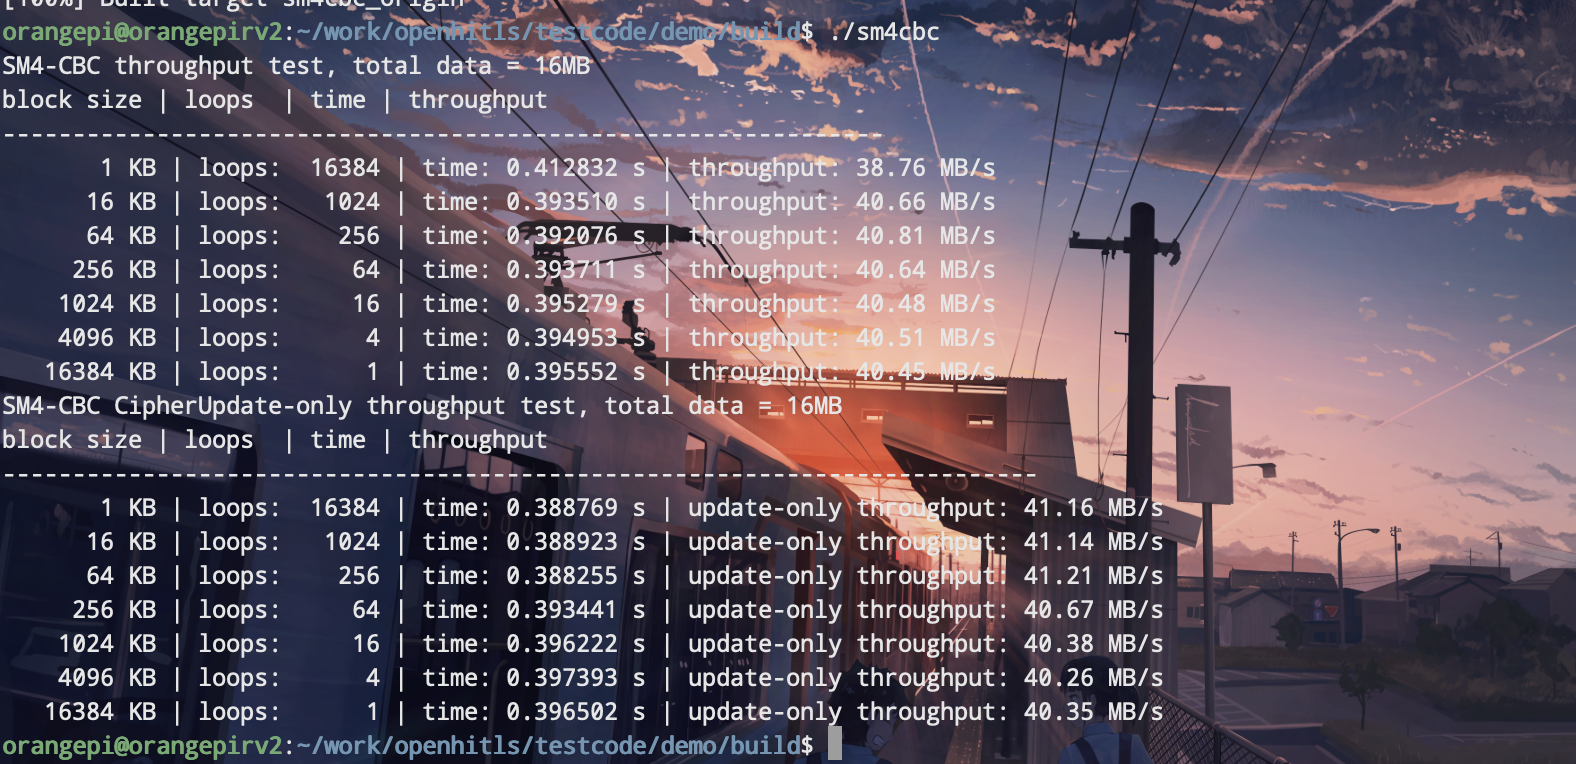
\includegraphics[width = 1\textwidth]{figure/openhitls_unrolled.png}
    \caption{openhitls SM4-CBC性能测试结果（循环展开优化）}
\end{figure}
不妨看16MB的吞吐率，由原来的39.09MB/s提升到了40.45MB/s
\subsubsection{Xbox合并}
在之前的实验中，我们已经实现了xbox优化方案，现在在openhitls中也进行相同的优化，修改如下:
\begin{lstlisting}[title={openhitls/crypto/sm4/src/crypt\_sm4.c}]
#define CRYPT_SM4_ROUND(t, x0, x1, x2, x3, rk)              \
    do {                                                    \
        (t) = (x1) ^ (x2) ^ (x3) ^ (rk);                    \
        (x0) ^= XBOX_3[((t) >> 24) & 0xff]                  \
              ^ XBOX_2[((t) >> 16) & 0xff]                  \
              ^ XBOX_1[((t) >> 8) & 0xff]                   \
              ^ XBOX_0[(t) & 0xff];                         \
    } while (0)
\end{lstlisting}
删除ENC\_ROUND\_FUNCTION等中的sbox参数
然后重新编译
运行测试程序，结果如下图:
\begin{figure}[H]
    \centering
    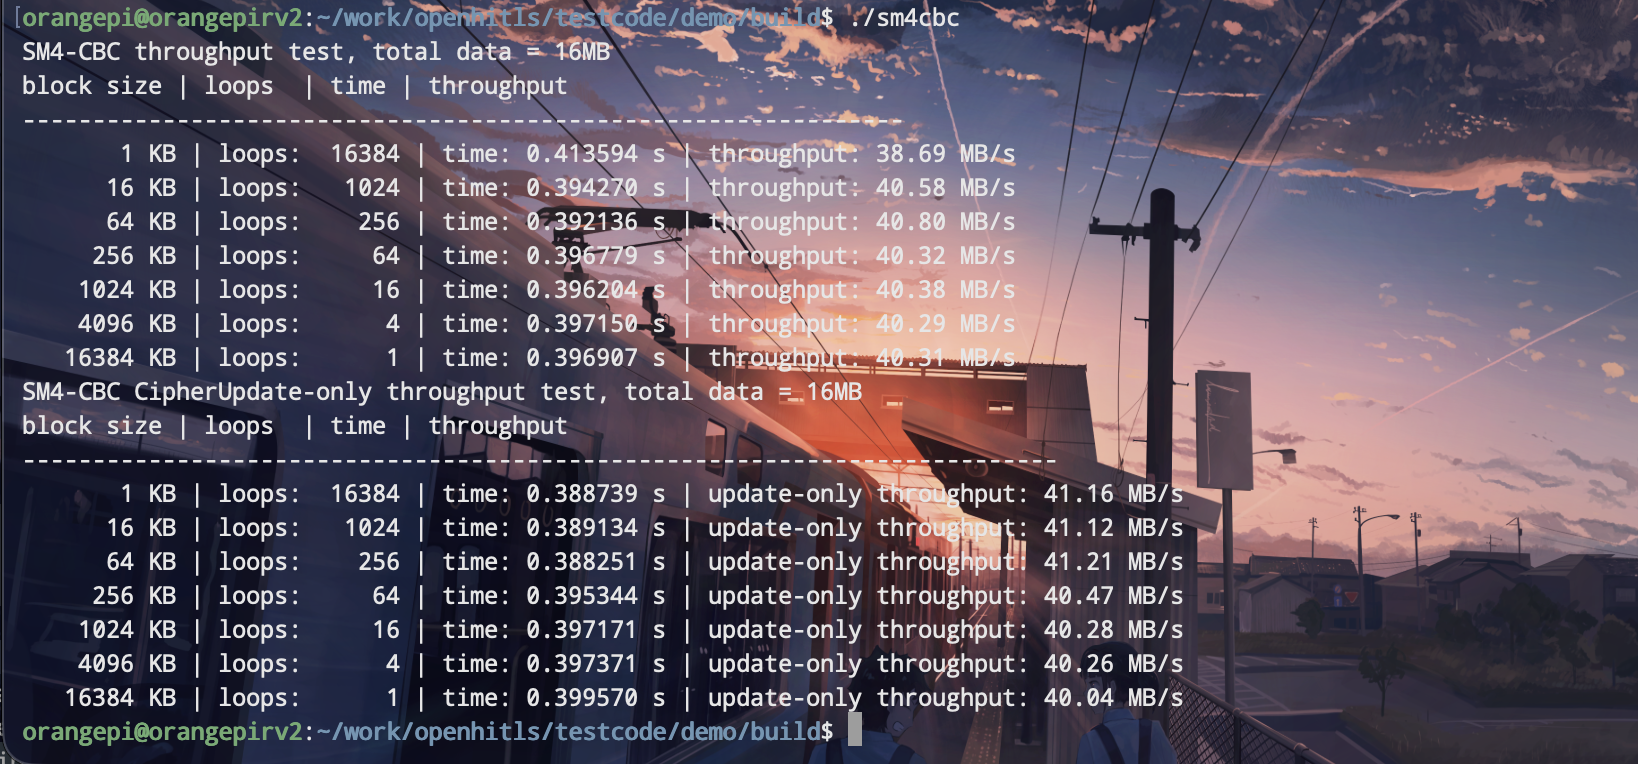
\includegraphics[width = 1\textwidth]{figure/openhitls_xbox.png}
    \caption{openhitls SM4-CBC性能测试结果（xbox合并优化）}
\end{figure}
\subsubsection{减少指令依赖优化}
在之前的实验中，我们已经实现了减少指令依赖优化方案，现在在openhitls中也进行相同的优化，修改如下:
\begin{lstlisting}[title={openhitls/crypto/sm4/src/crypt\_sm4.c}]
#define CRYPT_SM4_ROUND(t, x0, x1, x2, x3, rk)          \
    do {                                                \
        uint32_t t1 = (x1) ^ (x2);                      \
        uint32_t t2 = (x3) ^ (rk);                      \
        uint32_t te;                                    \
        (t) = t1 ^ t2;                                  \
        te = XBOX_3[((t) >> 24) & 0xff]                 \
           ^ XBOX_2[((t) >> 16) & 0xff]                 \
           ^ XBOX_1[((t) >> 8) & 0xff]                  \
           ^ XBOX_0[(t) & 0xff];                        \
        (x0) ^= te;                                     \
    } while (0)
\end{lstlisting}
然后重新编译
运行测试程序，结果如下图:
\begin{figure}[H]
    \centering
    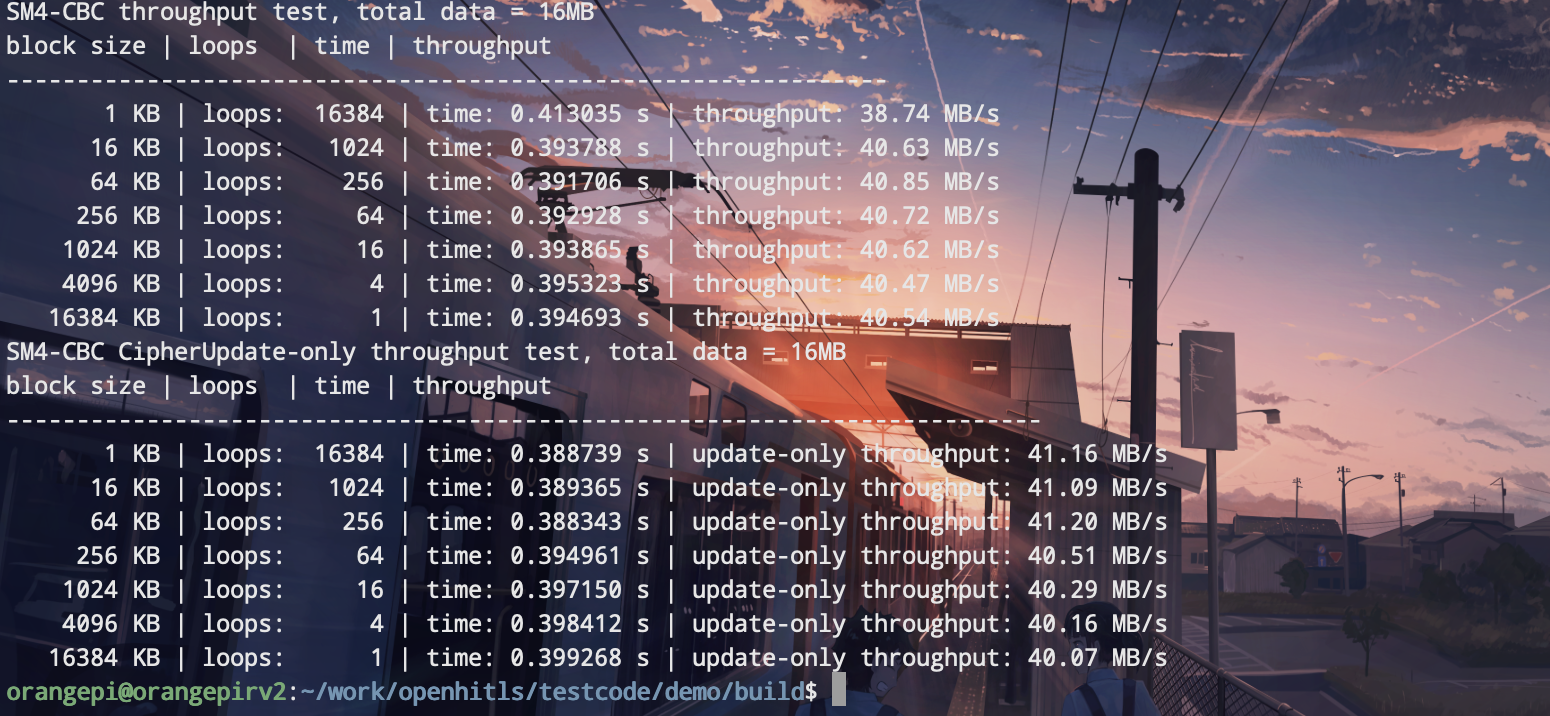
\includegraphics[width = 1\textwidth]{figure/openhitls_reduce_dep.png}
    \caption{openhitls SM4-CBC性能测试结果（减少指令依赖优化）}
\end{figure}

\subsubsection{默认字节序转换与 RISC-V B 拓展 rev8 转换}
用以下命令编译
\begin{lstlisting}
    cd ~/work/openhitls/build
    cmake .. \
  -DCMAKE_BUILD_TYPE=Release \
  -DCMAKE_C_FLAGS="-O3 -march=rv64gc_zba_zbb_zbs -mabi=lp64d -Wno-error -Wno-error=stringop-overflow -Wno-stringop-overflow" \
  -DCMAKE_C_FLAGS_RELEASE="-O3 -march=rv64gc_zba_zbb_zbs -mabi=lp64d -Wno-error -Wno-error=stringop-overflow -Wno-stringop-overflow"
    make -j$(nproc)
\end{lstlisting}
运行测试程序，结果如下图:
\begin{figure}[H]
    \centering
    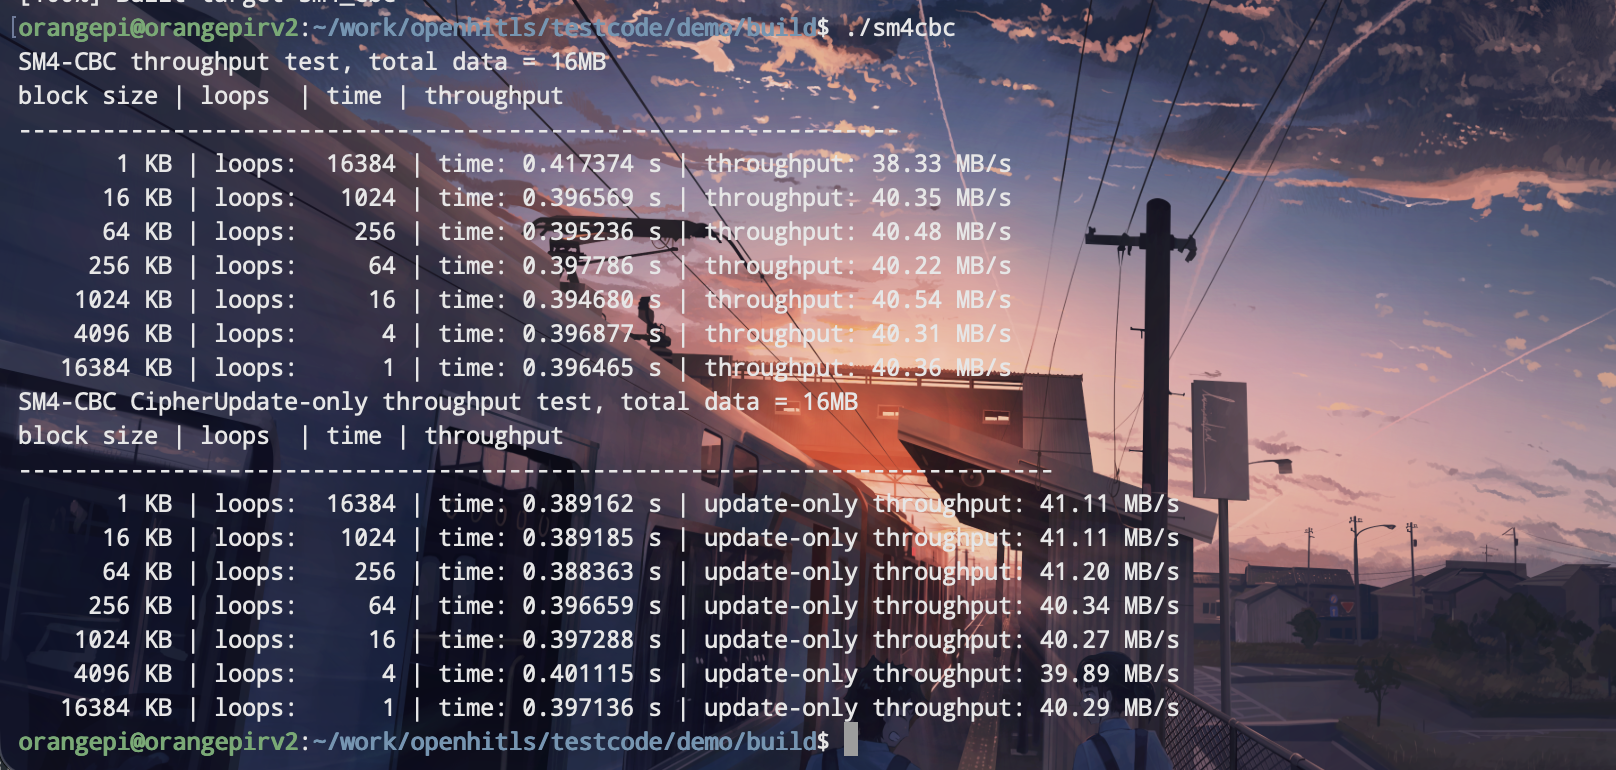
\includegraphics[width = 1\textwidth]{figure/openhitls_riscv_extend.png}
    \caption{openhitls SM4-CBC性能测试结果（RISC-V B 拓展 rev8 转换优化）}
\end{figure}

\subsubsection{总结}
可以看到在除了循环展开，其他方式似乎并没有带来太大的提升，这可能是由于openhitls的代码已经经过了较为充分的优化，进一步的优化空间较小。

\section{实验总结}

综合以上实验结果与分析,可以得到以下结论:

\begin{enumerate}
    \item \textbf{预计算查表是本实验中效果最显著的软件优化方式。}
    
    \texttt{xbox}方案通过预计算单字节对轮函数的贡献,取得了$1.2750\times$的几何平均加速比;\texttt{xbox\_merged}进一步使用4张预旋转查找表消除运行时循环移位操作,几何平均加速比达到$1.6115\times$,为本实验中性能最优的方案。这说明对于SM4轮函数,采用空间换时间的方式减少运行时计算具有较高收益。

    \item \textbf{局部指令级优化能够带来稳定但有限的性能提升。}
    
    循环展开方案\texttt{unrolled}和启用Zbb扩展的\texttt{zbb\_default}分别取得了$1.1224\times$和$1.1277\times$的几何平均加速比。相比之下,\texttt{reduced\_dep}的几何平均加速比仅为$1.0007\times$,几乎没有可观测收益。这说明局部代码重排或指令替换是否有效,取决于其是否真正作用于程序的关键路径。

    \item \textbf{不同优化策略叠加后并不一定产生线性增益。}
    
    \texttt{zbb\_xbox}在合并查表方案的基础上进一步启用了Zbb扩展,但其几何平均加速比为$1.5907\times$,略低于\texttt{xbox\_merged}的$1.6115\times$。原因在于合并查表已经消除了大部分运行时循环移位操作,使\texttt{rori}等位操作指令能够继续发挥作用的空间明显缩小。因此,优化策略之间可能存在功能重叠,实际效果还会受到编译器指令选择、寄存器分配和缓存访问行为等因素影响。

    \item \textbf{输入规模增大后,各方案吞吐率均有所下降。}
    
    其中,\texttt{default\_loop}从1 KB到16 MB的吞吐率下降约3.49\%,而\texttt{xbox\_merged}和\texttt{zbb\_xbox}分别下降约11.43\%和11.68\%。这说明查表方案虽然在全部测试规模下仍保持明显优势,但对输入规模变化更加敏感。该现象可能与缓存层次结构、流式数据加载与写回开销以及系统运行状态共同相关。

    \item \textbf{工程实现中应综合考虑性能收益与资源开销。}
    
    \texttt{xbox\_merged}需要额外存储4张查找表,空间开销为4 KB。对于本实验使用的Orange Pi RV2开发板,每核心具有32 KiB的L1数据缓存,因此该额外开销处于可接受范围。在类似资源条件下,建议优先采用\texttt{xbox\_merged}方案;在缓存和存储空间更加受限的平台上,则应根据实际资源约束在性能与空间之间进行权衡。
\end{enumerate}
